\documentclass[a4paper,landscape]{article}
\usepackage{lmodern}
\usepackage[margin=0.25cm]{geometry}
\usepackage{multicol}
\usepackage{tcolorbox}
\usepackage{amsmath} 
\pagestyle{empty}
\usepackage{algpseudocode}
\usepackage{algorithm} % For the algorithm environment
\usepackage{amssymb} % For math symbols
\usepackage{enumitem}
\usepackage{graphicx}
\usepackage{paracol}

\setlength{\parskip}{0pt}
\setlength{\baselineskip}{0pt}
\setlength{\columnsep}{0cm}
\setlength{\multicolsep}{0pt}
\setlist[itemize]{leftmargin=10pt,noitemsep,itemsep=0pt,nosep}
\setlist[enumerate]
{leftmargin=10pt,noitemsep,itemsep=0pt}

% Optional: Define a reusable box style
\tcbset{
  mybox/.style={
    colback=white,
    colframe=black,
    boxrule=0.5pt,
    arc=2pt,
    fonttitle=\bfseries\tiny,   % smaller title font size
    title={#1},
    left=0.1mm,
    right=0.1mm,
    top=0.1mm,
    bottom=0.1mm,
    boxrule=0.5pt,
    boxsep=0pt,
    before skip=0pt,
    after skip=0pt,
    before upper={%
      \tiny
      \setlength{\parskip}{0pt}%
      \setlength{\baselineskip}{0pt}%
      \setlength{\abovedisplayskip}{0pt}%
      \setlength{\belowdisplayskip}{0pt}%
      \setlength{\abovedisplayshortskip}{0pt}%
      \setlength{\belowdisplayshortskip}{0pt}%
    },
    before lower={%
      \tiny
      \setlength{\parskip}{0pt}%
      \setlength{\baselineskip}{0pt}%
      \setlength{\abovedisplayskip}{0pt}%
      \setlength{\belowdisplayskip}{0pt}%
      \setlength{\abovedisplayshortskip}{0pt}%
      \setlength{\belowdisplayshortskip}{0pt}%
    }
  }
}

% Command to color time complexity for readability
\newcommand{\timecomplexity}[1]{\textcolor{red}{#1}}
\newcommand{\bigo}{\mathcal{O}}
\algnewcommand{\LeftComment}[1]{\Statex \(\triangleright\) #1}

\begin{document}
\begin{multicols}{7} % Adjust number of columns as needed
\tcolorbox[mybox={Facts}]
\resizebox{0.75\textwidth}{!}{$\displaystyle \sum_{k=0}^{n} ar^k = \frac{ar^{n+1}-a}{r-1} \quad \text{for } r \notin \{0, 1\}$}

\tcblower

$\bigo(1)<\bigo((logn)^c)<\bigo(logn)\\<\bigo(log^2n)<\bigo(n)<\bigo(nlogn)\\<\bigo(n^c)<\bigo(c^n)<\bigo(n!)<\bigo(n^n)$

\endtcolorbox

\tcolorbox[mybox={Loop Invariant}]
A property that holds before and after each loop iteration.\\
\textbf{Initialization}: Holds before the first iteration.\\
\textbf{Maintenance}: If it holds before an iteration, it holds after.\\
\textbf{Termination}: When the loop ends, the invariant helps prove correctness.
\endtcolorbox
\tcolorbox[mybox={Divide and Conquer}]
An algorithmic paradigm with three steps:

1. \textbf{Divide}: Split the problem into smaller subproblems.\\
2. \textbf{Conquer}: Solve each subproblem recursively.\\
3. \textbf{Combine}: Merge the subproblem solutions into the final result.
The recurrence relation is:
\[
\scalebox{0.70}{$
T(n) =
\begin{cases}
\Theta(1) & \text{if } n \leq c, \\
a\,T(n/b) + D(n) + C(n) & \text{otherwise},
\end{cases}
$}
\]
\scalebox{0.7}{%
  \begin{minipage}{.9\linewidth}
  \raggedright
  \( a \): number of subproblems,\\
  \( n/b \): size of each subproblem,\\
  \( D(n) \): time to divide,\\
  \( C(n) \): time to combine.
  \end{minipage}
}
\endtcolorbox

\tcolorbox[mybox={Solving Recurrences}]
To solve a recurrence using the substitution method:

1. \textbf{Guess} the solution's form (e.g., \( \Theta(n^2) \)).\\
2. \textbf{Prove the upper bound} by induction using a constant and the guessed form.\\
  \textbf{Base cases:} For any constant $n \in \left\{2,3,4\right\}$, $T(n)$ has a constant value, selecting a larger than this value will satisfy the base cases when $n \in \left\{2,3,4\right\}$. \\
  \textbf{Inductive step:} Assume statement true $\forall n \in \left\{2,3,...,k-1\right\}$ and prove the statement for $n=k$.
  \begin{equation}
  \begin{split}
    T(n) & = 2T(n/2) + cn \\[-1mm]
    & \leq 2\frac{an}{2}log(n/2)+cn \\[-1mm]
    & = anlogn-an+cn \\[-1mm]
    & \leq anlogn \\[-1mm]
    & = \bigo(nlogn)
  \end{split}
  \end{equation}
  We can thus select a to be a positive constant so that both the base cases and the inductive step holds. \\Hence, $T(n)=\bigo(nlogn)$.\\
3. \textbf{Prove the lower bound} similarly.\\
4. \textbf{Conclude} that the guess is correct.
\textbf{Example:}\\
\( T(n) = T(n - 1) + cn \Rightarrow \Theta(n^2) \)
\endtcolorbox

\tcolorbox[mybox={Master Theorem}]
Let \( a \geq 1 \), \( b > 1 \), and let \( T(n) \) be defined by the recurrence:
\[T(n) = a\,T(n/b) + f(n)\]
Then \( T(n) \) has the following asymptotic bounds:
\begin{enumerate}[noitemsep, topsep=0pt]
    \item If \( f(n) = O(n^{\log_b a - \varepsilon}) \) \\ for some \( \varepsilon > 0 \),\\
          then \( T(n) = \Theta(n^{\log_b a}) \).

    \item If \( f(n) = \Theta(n^{\log_b a}) \),
          then \\ \( T(n)=\Theta(n^{\log_b a}logn) \).

    \item If \( f(n) = \Omega(n^{\log_b a + \varepsilon}) \) \\ for some \( \varepsilon > 0 \),\\
          and if \( a\,f(n/b) \leq c\,f(n) \) \\ for some \( c < 1 \) and large \( n \),\\
          then \( T(n) = \Theta(f(n)) \).
\end{enumerate}
\tcblower
Special case:\\
\(T(n) = a_1T(b_1n) + a_2T(b_2n) + ... + n^c\)
\begin{enumerate}[noitemsep, topsep=0pt]
    \item If \(a_1b_1^c + a_2b_2^c + ...  < 1 \) \\ \hspace*{2mm} then \( \Theta(n^c)\).
    \item If \(a_1b_1^c + a_2b_2^c + ...  = 1\) \\ \hspace*{2mm} then \( \Theta(n^c \log n)\).
    \item If \(a_1b_1^c + a_2b_2^c + ...  > 1 \) \\ \hspace*{2mm} then \( \Theta(n^e)\), \\ \hspace*{2mm} where \(a_1b_1^e + a_2b_2^e + ... = 1\).
\end{enumerate}
\endtcolorbox

\tcolorbox[mybox={Injective Functions}] 
Let $f : \{1, 2, \dots, q\} \to M$ be a function chosen uniformly at random, where $|M| = m$.  
If $q > 1.78\sqrt{m}$, then the probability that $f$ is injective is at most $\frac{1}{2}$.\\
$q$ = N\# inputs and $m$ = N\# outputs.
\endtcolorbox

\tcolorbox[mybox={Insertion Sort}]
\textbf{Steps:}
\begin{enumerate}[noitemsep, topsep=0pt]
    \item Start with an empty (or trivially sorted) sublist.
    \item Insert the next element in the correct position by comparing backwards.
    \item Repeat for all elements.
\end{enumerate}
\textbf{Complexity:}\\
Time: \timecomplexity{\( \Theta(n^2) \)}, Space: \( \Theta(n) \)\\
\textbf{Pseudocode:}
\noindent % Prevents indentation if at the start of a paragraph
\resizebox{\linewidth}{!}{%
\begin{minipage}{\linewidth}
\begin{algorithmic}[1]
    \Require $A = \langle a_1, a_2, \dots, a_n \rangle$
    \For{$i \gets 2$ to $n$}
        \State \textit{key} $\gets A[i]$
        \State $j \gets i - 1$
        \While{$j \geq 1$ and $A[j] > \textit{key}$}
            \State $A[j + 1] \gets A[j]$
            \State $j \gets j - 1$
        \EndWhile
        \State $A[j + 1] \gets \textit{key}$
    \EndFor
\end{algorithmic}
\end{minipage}%
}
\endtcolorbox

\tcolorbox[mybox={Heap Sort}]
A heap is a \textbf{nearly complete binary tree} where each node satisfies the \textbf{max-heap property}:
For every node i, its children have smaller or equal values.

The \textbf{height} of a heap is the length of the longest path from the root to a leaf.

\textbf{Useful Index Rules (array-based heap):}
\begin{itemize}[noitemsep, topsep=0pt]
    \item Root is at index \( A[1] \)
    \item Left child of node \( i \): index \( 2i \)
    \item Right child of node \( i \): index \( 2i + 1 \)
    \item Parent of node \( i \): index \( \lfloor i/2 \rfloor \)
\end{itemize}

\textbf{Complexity:} \\
Time: \timecomplexity{\( \Theta(n \log n) \)}, Space: \( \Theta(n) \) \\
\textbf{Pseudocode:}\\
\noindent % Prevents indentation if at the start of a paragraph
\resizebox{\linewidth}{!}{%
\begin{minipage}{1.25\linewidth}
\begin{algorithmic}[1]
    \Procedure{Max-Heapify}{$A, i, n$} \timecomplexity{$\bigo(logn)$}
        \State $l \gets \text{Left}(i)$
        \State $r \gets \text{Right}(i)$
        \State \textit{largest} $\gets i$
        \If{$l \leq n$ and $A[l] > A[\textit{largest}]$}
            \State \textit{largest} $\gets l$
        \EndIf
        \If{$r \leq n$ and $A[r] > A[\textit{largest}]$}
            \State \textit{largest} $\gets r$
        \EndIf
        \If{\textit{largest} $\neq i$}
            \State Exchange $A[i] \leftrightarrow A[\textit{largest}]$
            \State \Call{Max-Heapify}{$A, \textit{largest}, n$}
        \EndIf
    \EndProcedure
\end{algorithmic}
\end{minipage}%
}

\vspace{1em} % Add some vertical space between algorithms for better separation

\noindent % Prevents indentation if at the start of a paragraph
\resizebox{\linewidth}{!}{%
\begin{minipage}{1.25\linewidth}
\begin{algorithmic}[1]
    \Procedure{Build-Max-Heap}{$A[1, \dots, n]$} \timecomplexity{$\bigo(n)$}
        \For{$i \gets \lfloor n/2 \rfloor \text{ downto } 1$}
            \State \Call{Max-Heapify}{$A, i, n$}
        \EndFor
    \EndProcedure
\end{algorithmic}
\end{minipage}%
}

\vspace{1em} % Add some vertical space between algorithms for better separation

\noindent % Prevents indentation if at the start of a paragraph
\resizebox{\linewidth}{!}{%
\begin{minipage}{1.25\linewidth}
\begin{algorithmic}[1]
    \Procedure{Heapsort}{$A[1, \dots, n]$} \timecomplexity{$\bigo(nlogn)$}
        \State \Call{Build-Max-Heap}{$A$}
        \For{$i \gets n \text{ downto } 2$}
            \State exchange $A[1]$ with $A[i]$
            \State \Call{Max-Heapify}{$A, 1, i - 1$}
        \EndFor
    \EndProcedure
\end{algorithmic}
\end{minipage}%
}
\endtcolorbox

\tcolorbox[mybox={Merge Sort}]
Uses the \textbf{divide and conquer} paradigm. \\
\textbf{Complexity:}\\
Time: \timecomplexity{\( \Theta(n \log n) \)}, Space: \( \Theta(n) \) \\
\textbf{Pseudocode:}
\noindent % Prevents indentation if at the start of a paragraph
\resizebox{\linewidth}{!}{%
\begin{minipage}{1.25\linewidth}
\begin{algorithmic}[1]
    \Procedure{sort}{$A, p, r$}
        \If{$p < r$}
            \State $q \gets \lfloor (p + r)/2 \rfloor$
            \State \Call{sort}{$A, p, q$}
            \State \Call{sort}{$A, q + 1, r$}
            \State \Call{merge}{$A, p, q, r$}
        \EndIf
    \EndProcedure
\end{algorithmic}
\end{minipage}%
}

\vspace{1em} % Add some vertical space between algorithms for better separation

\noindent % Prevents indentation if at the start of a paragraph
\resizebox{\linewidth}{!}{%
\begin{minipage}{1.25\linewidth}
\begin{algorithmic}[1]
    \Procedure{merge}{$A, p, q, r$}
        \State $n_1 \gets q - p + 1$, $n_2 \gets r - q$
        \State Let $L[1 \dots n_1 + 1]$, $R[1 \dots n_2 + 1]$ be new arrays
        \For{$i \gets 1$ to $n_1$} $L[i] \gets A[p + i - 1]$ \EndFor
        \For{$j \gets 1$ to $n_2$} $R[j] \gets A[q + j]$ \EndFor
        \State $L[n_1 + 1], R[n_2 + 1] \gets \infty$
        \State $i, j \gets 1$
        \For{$k \gets p$ to $r$}
            \If{$L[i] \leq R[j]$}
                \State $A[k] \gets L[i]$; $i \gets i + 1$
            \Else
                \State $A[k] \gets R[j]$; $j \gets j + 1$
            \EndIf
        \EndFor
    \EndProcedure
\end{algorithmic}
\end{minipage}%
}
\endtcolorbox

\tcolorbox[mybox={Stack}]
A stack is a last-in/fist-out (LIFO) data-structure\\
\textbf{Supported operations:}
\begin{itemize}[noitemsep,itemsep=0pt]
    \item \textbf{Push:} Insert an element at head. \timecomplexity{\(\bigo(1)\)}
    \item \textbf{Pop:} Retrieve head. \timecomplexity{\(\bigo(1)\)}
\end{itemize}
\endtcolorbox

\tcolorbox[mybox={Maximum Subarray Problem (Kadane's Algorithm)}]
\textbf{Idea:}
Iterate from left to right, maintaining:
- \texttt{endingHereMax}: best subarray ending at current index
- \texttt{currentMax}: best seen so far

\textbf{Observation:}
At index \( j+1 \), the maximum subarray is either:
\begin{itemize}[noitemsep,itemsep=0pt]
    \item the best subarray in \( A[1..j] \), or
    \item a subarray ending at \( j+1 \), i.e., \( A[i..j+1] \)
\end{itemize}
\textbf{Formula:}
\[
\resizebox{1\textwidth}{!}{$
    \text{maxSub}(A[1..n]) = \max\left(
    \text{maxSub}(A[1..n-1]),\ 
    \max_{i=1}^{n} \text{sum}(A[i..n])
    \right)
$}
\]
\textbf{Complexity:} \\
Time: \timecomplexity{\( \Theta(nlogn) \)}, Space: \( \Theta(n) \)\\
\textbf{Pseudocode:}
\resizebox{\linewidth}{!}{%
\begin{minipage}{1.25\linewidth}
\begin{algorithmic}[1]
\Procedure{Linear-Max-Subarray}{$A[1..n]$} 
    \State $current\_max \gets -\infty$
    \State $ending\_here\_max \gets -\infty$
    \For{$i \gets 1$ to $n$}
        \State $ending\_here\_max \gets \max(A[i], ending\_here\_max + A[i])$
        \State $current\_max \gets \max(current\_max, ending\_here\_max)$
    \EndFor
    \State \Return $current\_max$
\EndProcedure
\end{algorithmic}
\end{minipage}
}

\endtcolorbox
\tcolorbox[mybox={Queue}]
A queue is a first-in, first-out (FIFO) collection.
\begin{itemize}[noitemsep,itemsep=0pt]
    \item \textbf{enqueue:} Insert an element at tail. \timecomplexity{\(\bigo(1)\)}
    \item \textbf{dequeue:} Retrieve head. \timecomplexity{\(\bigo(1)\)}
\end{itemize}
\begin{algorithmic}[1]
    \Procedure{Enqueue}{$Q, x$}
        \State $Q[Q.\text{tail}] \gets x$
        \If{$Q.\text{tail} = Q.\text{length}$}
            \State $Q.\text{tail} \gets 1$
        \Else
            \State $Q.\text{tail} \gets Q.\text{tail} + 1$
        \EndIf
    \EndProcedure
    \State
    \Procedure{Dequeue}{$Q$}
        \State $x \gets Q[Q.\text{head}]$
        \If{$Q.\text{head} = Q.\text{length}$}
            \State $Q.\text{head} \gets 1$
        \Else
            \State $Q.\text{head} \gets Q.\text{head} + 1$
        \EndIf
        \State \Return $x$
    \EndProcedure
\end{algorithmic}
\endtcolorbox

\tcolorbox[mybox={Dynamic Programming}]
Two key approaches: \textbf{Top-down} and \textbf{Bottom-up}.
\begin{itemize}[noitemsep, itemsep=0pt]
    \item \textbf{Top-down:} Starts from the problem $n$ and solves subproblems recursively, storing results (memoization).
    \item \textbf{Bottom-up:} Starts from base cases (e.g., 0) and iteratively builds up to the final solution.
\end{itemize}
The core idea is to \textbf{remember previous computations} to avoid redundant work and save time.
\endtcolorbox

\tcolorbox[mybox={Binary search}]
\begin{algorithmic}[1]
    \Procedure{BS}{$A,k,p,q$}
        \If{$q<p$}
            \State \Return $"NO"$ \Comment{array is empty and doesn't contain k}
        \Else
            \State $mid \gets \lfloor \frac{p+q}{2} \rfloor$
            \If{$A[mid] = k$}
                \State \Return $"YES"$
            \ElsIf{$A[mid] > k$}
                \State \Return \Call{BS}{$A,k,p,mid-1$}
            \Else
                \State \Return \Call{BS}{$A,k,mid+1,q$}
            \EndIf
        \EndIf
    \EndProcedure
\end{algorithmic}
\textbf{Time complexity:} \timecomplexity{$\bigo(logn)$}
\endtcolorbox

\tcolorbox[mybox={Strassen’s Algorithm for Matrix Multiplication}]
Instead of performing 8 recursive multiplications as in the naive divide-and-conquer matrix multiplication, Strassen’s algorithm reduces it to 7, which improves the time complexity.\\
\textbf{\strut Definitions:}
\begin{align*}
M_1 &= (A_{11} + A_{22})(B_{11} + B_{22}) \\
M_2 &= (A_{21} + A_{22})B_{11} \\
M_3 &= A_{11}(B_{12} - B_{22}) \\
M_4 &= A_{22}(B_{21} - B_{11}) \\
M_5 &= (A_{11} + A_{12})B_{22} \\
M_6 &= (A_{21} - A_{11})(B_{11} + B_{12}) \\
M_7 &= (A_{12} - A_{22})(B_{21} + B_{22})
\end{align*}
\textbf{Resulting matrix:}
\begin{align*}
C_{11} &= M_1 + M_4 - M_5 + M_7 \\
C_{12} &= M_3 + M_5 \\
C_{21} &= M_2 + M_4 \\
C_{22} &= M_1 - M_2 + M_3 + M_6
\end{align*}
\textbf{Recursion:} $T(n) = 7T(n/2) + \Theta(n^2)$
\textbf{Complexity:} \\
Time: \timecomplexity{\( \Theta(n^{\log_2 7}) \approx \Theta(n^{2.81}) \)} \\ Space: \( \Theta(n^2) \)
\endtcolorbox

\tcolorbox[mybox={Priority Queue}]
A priority queue maintains a dynamic set \( S \) of elements, each with an associated key that defines its priority. At each operation, we can access the element with the highest key. \\
\textbf{Supported operations:}
\begin{itemize}[noitemsep,itemsep=0pt]
    \item \textbf{Insertion:} Insert an element \( x \) into \( S \). \timecomplexity{\(\bigo(log(n))\)}
    \item \textbf{Maximum:} Return the element in \( S \) with the largest key. \timecomplexity{\(\Theta(1)\)}
    \item \textbf{Extract-Max:} Remove and return the element with the largest key. \timecomplexity{\(\bigo(log(n))\)}
    \item \textbf{Increase-Key:} Increase the key of an element \( x \) to a new value \( k \) (assuming \( k \geq \) current key). \timecomplexity{\(\bigo(log(n))\)}
\end{itemize}

\textbf{Pseudocode:}
    \noindent % Prevents indentation if at the start of a paragraph
\resizebox{\linewidth}{!}{%
\begin{minipage}{1.25\linewidth}
\begin{algorithmic}[1]
      \Procedure{Heap-Maximum}{$S$}
        \State \Return $S[1]$
      \EndProcedure
\end{algorithmic}
\end{minipage}%
}

\noindent % Prevents indentation if at the start of a paragraph
\resizebox{\linewidth}{!}{%
\begin{minipage}{1.25\linewidth}
\begin{algorithmic}[1]
      \Procedure{Heap-Extract-Max}{$S, n$}
        \If{$n < 1$}
          \State \textbf{error} "heap underflow"
        \EndIf
        \State $max \gets S[1]$
        \State $S[1] \gets S[n]$
        \State $n \gets n - 1$
        \State \Call{Max-Heapify}{$S, 1, n$}
        \State \Return $max$
      \EndProcedure
\end{algorithmic}
\end{minipage}%
}
\noindent % Prevents indentation if at the start of a paragraph
\resizebox{\linewidth}{!}{%
\begin{minipage}{1.25\linewidth}
\begin{algorithmic}[1]
      \Procedure{Heap-Increase-Key}{$S, i, key$}
        \If{$key < S[i]$}
          \State \textbf{error} "new key is smaller than current key"
        \EndIf
        \State $S[i] \gets key$
        \While{$i > 1$ \textbf{and} $S[\text{Parent}(i)] < S[i]$}
          \State exchange $S[i]$ with $S[\text{Parent}(i)]$
          \State $i \gets \text{Parent}(i)$
        \EndWhile
      \EndProcedure
\end{algorithmic}
\end{minipage}%
}
\noindent % Prevents indentation if at the start of a paragraph
\resizebox{\linewidth}{!}{%
\begin{minipage}{1.25\linewidth}
\begin{algorithmic}[1]
    \Procedure{Max-Heap-Insert}{$S, key, n$}
        \State $n \gets n + 1$
        \State $S[n] \gets -\infty$
        \State \Call{Heap-Increase-Key}{$S, n, key$}
    \EndProcedure
\end{algorithmic}
\end{minipage}%
}
\endtcolorbox

\tcolorbox[mybox={Disjoint sets}]
\begin{itemize}[noitemsep,itemsep=0pt]
    \item \(S = {S_1, ..., S_k}\) is a collection of disjoint dynamic sets. Each set is identified by a representative which is a member of the set.
    \item Uses a \timecomplexity{linked list} or a \textcolor{blue}{graph forest}.
    \item \textbf{Make-Set(x):} make a new set \(S_i = {x}\) and add $S_i$ to $S$. \timecomplexity{\(\Theta(1)\)} \textcolor{blue}{\(\Theta(1)\)}
    \item \textbf{Union(x,y):} if \(x \in S_x, y \in S_y\) then \(S = S - S_x - S_y \cup {S_x \cup S_y}\). \timecomplexity{\(\bigo(m+nlogn)\)} \textcolor{blue}{\(\bigo(m \alpha(n))\)}
    \item \textbf{Find(x):} returns the representative of the set containing x. \timecomplexity{\(\Theta(1)\)} \textcolor{blue}{\(\bigo(h)\)}
    \item \textbf{Connected components:} returns disjoint sets of all vertices connected inside a graph. \\ \timecomplexity{\(\bigo(VlogV + E)\)} \textcolor{blue}{\(\bigo(V+E)\)}
\end{itemize}
\endtcolorbox

\tcolorbox[mybox={Linked List}]
A linked list is a linear data structure where each element (node) points to the next. Unlike arrays, it is not index-based and allows efficient insertions and deletions.

\textbf{Operations:}
\begin{itemize}[noitemsep,itemsep=0pt]
    \item \textbf{Search:} Find an element with a specific key \timecomplexity{\(\bigo(n)\)}
    \item \textbf{Insert:} Insert an element at the head \timecomplexity{\(\Theta(1)\)}
    \item \textbf{Delete:} Remove an element \timecomplexity{\(\Theta(1)\)} \\ \timecomplexity{$\bigo(n)$} if simple list
\end{itemize}

\textbf{Pseudocode:}

\noindent % Prevents indentation if at the start of a paragraph
\resizebox{\linewidth}{!}{%
\begin{minipage}{1.5\linewidth}
\begin{algorithmic}[1]
    \LeftComment{Searches for the first element with key $k$}
    \Procedure{List-Search}{$L, k$}
        \State $x \gets L.\text{head}$
        \While{$x \neq \text{NIL}$ \textbf{and} $x.\text{key} \neq k$}
            \State $x \gets x.\text{next}$
        \EndWhile
        \State \Return $x$
    \EndProcedure

    \LeftComment{Inserts a new node $x$ at the head of the list}
    \Procedure{List-Insert}{$L, x$}
        \State $x.\text{next} \gets L.\text{head}$
        \If{$L.\text{head} \neq \text{NIL}$}
            \State $L.\text{head}.\text{prev} \gets x$
        \EndIf
        \State $L.\text{head} \gets x$
        \State $x.\text{prev} \gets \text{NIL}$
    \EndProcedure

    \LeftComment{Deletes node $x$ from the list}
    \Procedure{List-Delete}{$L, x$}
        \If{$x.\text{prev} \neq \text{NIL}$}
            \State $x.\text{prev}.\text{next} \gets x.\text{next}$
        \Else
            \State $L.\text{head} \gets x.\text{next}$
        \EndIf
        \If{$x.\text{next} \neq \text{NIL}$}
            \State $x.\text{next}.\text{prev} \gets x.\text{prev}$
        \EndIf
    \EndProcedure
\end{algorithmic}
\end{minipage}%
}
\endtcolorbox

\tcolorbox[mybox={Binary Search Trees}]
A binary search tree (BST) is a binary tree where each node has a key and satisfies the following properties:
\begin{itemize}[noitemsep, itemsep=0pt]
    \item For any node $x$, all keys in its left subtree are less than $x.\text{key}$.
    \item All keys in its right subtree are greater than or equal to $x.\text{key}$.
\end{itemize}

\textbf{Pseudocode:}

\noindent % Prevents indentation if at the start of a paragraph
\resizebox{\linewidth}{!}{%
\begin{minipage}{1.25\linewidth}
\begin{algorithmic}[1]
    \LeftComment{Searches for a node with key $k$ starting from node $x$}
    \Statex \Comment{Runs in \timecomplexity{$\bigo(h)$} time, where $h$ is the height of the tree ($\bigo(log(n))$ if balanced)}
    \Procedure{Tree-Search}{$x, k$}
        \If{$x = \text{NIL}$ \textbf{or} $k = x.\text{key}$}
            \State \Return $x$
        \ElsIf{$k < x.\text{key}$}
            \State \Return \Call{Tree-Search}{$x.\text{left}, k$}
        \Else
            \State \Return \Call{Tree-Search}{$x.\text{right}, k$}
        \EndIf
    \EndProcedure

    \Statex \Comment{Finds the minimum key node in the subtree rooted at $x$}
    \Procedure{Tree-Minimum}{$x$} \timecomplexity{$\bigo(h)$}
        \While{$x.\text{left} \neq \text{NIL}$}
            \State $x \gets x.\text{left}$
        \EndWhile
        \State \Return $x$
    \EndProcedure

    \Statex \Comment{Finds the maximum key node in the subtree rooted at $x$}
    \Procedure{Tree-Maximum}{$x$} \timecomplexity{$\bigo(h)$}
        \While{$x.\text{right} \neq \text{NIL}$}
            \State $x \gets x.\text{right}$
        \EndWhile
        \State \Return $x$
    \EndProcedure
\end{algorithmic}
\end{minipage}%
}
\endtcolorbox

\tcolorbox[mybox={Rod Cutting}]
Given a rod of length $n$ and a table of prices $p_i$ for rods of length $i = 1, \dots, n$, determine the optimal way to cut the rod to maximize profit.\\
The optimal revenue function $r(n)$ is defined as:
\resizebox{1\textwidth}{!}{$
r(n) =
\begin{cases}
    0 & \text{if } n = 0, \\
    \max_{1 \leq i \leq n} \{p_i + r(n - i)\} & \text{if } n \geq 1.
\end{cases}
$}

\noindent % Prevents indentation if at the start of a paragraph
\resizebox{\linewidth}{!}{%
\begin{minipage}{1.25\linewidth}
\begin{algorithmic}[1]
    \Procedure{Extended-Bottom-Up-Cut-Rod}{$p, n$}
        \State let $r[0 \dots n]$ and $s[0 \dots n]$ be new arrays
        \State $r[0] \gets 0$
        \State $s[0] \gets 0$ \Comment{Usually $s[0]$ isn't explicitly used for solution reconstruction, but included as per your pseudocode}
        \For{$j \gets 1 \text{ to } n$}
            \State $q \gets -\infty$
            \For{$i \gets 1 \text{ to } j$}
                \If{$q < p[i] + r[j - i]$}
                    \State $q \gets p[i] + r[j - i]$
                    \State $s[j] \gets i$
                \EndIf
            \EndFor
            \State $r[j] \gets q$
        \EndFor
        \State \Return $r \text{ and } s$
    \EndProcedure
\end{algorithmic}
\end{minipage}%
}
\textbf{Time complexity:} \timecomplexity{\(\Theta(n^2)\)} \\
Space complexitiy: $\bigo(n)$
\endtcolorbox

\tcolorbox[mybox={Modify a Binary Tree}]
\noindent % Prevents indentation if at the start of a paragraph
\resizebox{\linewidth}{!}{%
\begin{minipage}{1.25\linewidth}
$\triangleright$ With h being the height of the tree.
\begin{algorithmic}[1]
    \Procedure{Tree-Insert}{$T, z$} \timecomplexity{\(\bigo(h)\)}
        \State $y \gets \text{NIL}$ \Comment{Parent of $x$}
        \State $x \gets T.\text{root}$
        \While{$x \neq \text{NIL}$}
            \State $y \gets x$
            \If{$z.\text{key} < x.\text{key}$}
                \State $x \gets x.\text{left}$
            \Else
                \State $x \gets x.\text{right}$
            \EndIf
        \EndWhile
        \State $z.p \gets y$
        \If{$y = \text{NIL}$}
            \State $T.\text{root} \gets z$
        \ElsIf{$z.\text{key} < y.\text{key}$}
            \State $y.\text{left} \gets z$
        \Else
            \State $y.\text{right} \gets z$
        \EndIf
    \EndProcedure

    \Procedure{Transplant}{$T, u, v$} \timecomplexity{$\Theta(1)$}
        \If{$u.p = \text{NIL}$}
            \State $T.\text{root} \gets v$
        \ElsIf{$u = u.p.\text{left}$}
            \State $u.p.\text{left} \gets v$
        \Else
            \State $u.p.\text{right} \gets v$
        \EndIf
        \If{$v \neq \text{NIL}$}
            \State $v.p \gets u.p$
        \EndIf
    \EndProcedure

    \Procedure{Tree-Delete}{$T, z$} \timecomplexity{\(\bigo(h)\)}
        \If{$z.\text{left} = \text{NIL}$}
            \State \Call{Transplant}{$T, z, z.\text{right}$}
        \ElsIf{$z.\text{right} = \text{NIL}$}
            \State \Call{Transplant}{$T, z, z.\text{left}$}
        \Else
            \State $y \gets \Call{Tree-Minimum}{z.\text{right}}$
            \If{$y.p \neq z$}
                \State \Call{Transplant}{$T, y, y.\text{right}$}
                \State $y.\text{right} \gets z.\text{right}$
                \State $y.\text{right}.p \gets y$
            \EndIf
            \State \Call{Transplant}{$T, z, y$}
            \State $y.\text{left} \gets z.\text{left}$
            \State $y.\text{left}.p \gets y$
        \EndIf
    \EndProcedure

    \Procedure{Tree-Successor}{$x$} \timecomplexity{$\bigo(h)$}
        \If{$x.\text{right} \neq \text{NIL}$}
            \State \Return \Call{Tree-Minimum}{$x.\text{right}$}
        \EndIf
        \State $y \gets x.\text{p}$
        \While{$y \neq \text{NIL and } x == y.\text{right}$}
            \State $x \gets y$
            \State $y \gets y.\text{p}$
        \EndWhile
        \State \Return $y$
    \EndProcedure
\end{algorithmic}
\end{minipage}%
}

\tcblower
\resizebox{\linewidth}{!}{%
\begin{minipage}{1.25\linewidth}
\begin{algorithmic}[1]
    \Procedure{Inorder-Tree-Walk}{$x$} \timecomplexity{\(\bigo(n)\)}
        \If{$x \neq NIL$}
            \State \Call{Inorder-Tree-Walk}{$x.\text{left}$}
            \State print $key[x]$
            \State \Call{Inorder-Tree-Walk}{$x.\text{right}$}
        \EndIf
    \EndProcedure
\end{algorithmic}
$\triangleright$ Preorder: print - call(x.left) - call(x.right) \\
$\triangleright$ Postorder: call(x.left) - call(x.right) - print
\end{minipage}%
}
\endtcolorbox

\tcolorbox[mybox={Counting Sort}]
\textbf{Counting Sort} assumes the input consists of $n$ integers in the range $0$ to $k$ and sorts them in \timecomplexity{$\bigo(n + k)$} time. It is stable and non-comparative.

\noindent % Prevents indentation before the resizebox
\resizebox{\linewidth}{!}{%
\begin{minipage}{1.25\linewidth}
\begin{algorithmic}[1]
    \Procedure{Counting-Sort}{$A, B, n, k$}
        \State let $C[0 \dots k]$ be a new array
        \For{$i \gets 0$ \textbf{to} $k$}
            \State $C[i] \gets 0$
        \EndFor
        \For{$j \gets 1$ \textbf{to} $n$}
            \State $C[A[j]] \gets C[A[j]] + 1$
        \EndFor
        \For{$i \gets 1$ \textbf{to} $k$}
            \State $C[i] \gets C[i] + C[i - 1]$
        \EndFor
        \For{$j \gets n$ \textbf{downto} $1$}
            \State $B[C[A[j]]] \gets A[j]$
            \State $C[A[j]] \gets C[A[j]] - 1$
        \EndFor
    \EndProcedure
\end{algorithmic}
\end{minipage}%
}
\endtcolorbox

\tcolorbox[mybox={Building a Binary Search Tree}]
Given a sequence $K = \langle k_1, k_2, \dots, k_n \rangle$ of $n$ distinct sorted keys and, for every $k_i$, a probability $p_i$, find a binary search tree $T$ that minimizes:
\resizebox{0.95\linewidth}{!}{%
$\displaystyle
E[\text{search cost in } T] = \sum_{i=1}^{n} (\text{depth}_T (k_i) + 1)\cdot p_i
$%
}


This is solved via dynamic programming.

\textbf{Time complexity:} \timecomplexity{\(\bigo(n^3)\)}

\noindent % Prevents indentation before the resizebox
\resizebox{\linewidth}{!}{%
\begin{minipage}{1.25\linewidth}
\begin{algorithmic}[1]
    \Procedure{Optimal-BST}{$p, q, n$}
        \State let $e[1 \dots n+1][0 \dots n]$, $w[1 \dots n+1][0 \dots n]$, and $\text{root}[1 \dots n][1 \dots n]$ be new tables
        \For{$i \gets 1 \text{ to } n+1$}
            \State $e[i][i-1] \gets 0$
            \State $w[i][i-1] \gets 0$
        \EndFor
        \For{$l \gets 1 \text{ to } n$} \Comment{length of subproblem}
            \For{$i \gets 1 \text{ to } n - l + 1$}
                \State $j \gets i + l - 1$
                \State $e[i][j] \gets \infty$
                \State $w[i][j] \gets w[i][j-1] + p[j]$
                \For{$r \gets i \text{ to } j$}
                    \State $t \gets e[i][r-1] + e[r+1][j] + w[i][j]$
                    \If{$t < e[i][j]$}
                        \State $e[i][j] \gets t$
                        \State $\text{root}[i][j] \gets r$
                    \EndIf
                \EndFor
            \EndFor
        \EndFor
    \EndProcedure
\end{algorithmic}
\end{minipage}%
}
\endtcolorbox

\tcolorbox[mybox={Matrix-Chain Multiplication}]
Given a chain $\langle A_1, A_2, \dots, A_n \rangle$ of $n$ matrices, where for $i = 1, 2, \dots, n$, matrix $A_i$ has dimensions $p_{i-1} \times p_i$, find the most efficient way to fully parenthesize the product $A_1 A_2 \cdots A_n$ so as to minimize the total number of scalar multiplications.

The optimal substructure is defined by the recurrence:
\resizebox{1\textwidth}{!}{$
m[i, j] =
\begin{cases}
    0 & \text{if } i = j, \\
    \min_{i \leq k < j} \{m[i, k] + m[k + 1, j] + p_{i-1} p_k p_j\} & \text{if } i < j.
\end{cases}
$}

\resizebox{\linewidth}{!}{%
\begin{minipage}{1.25\linewidth}
\begin{algorithmic}[1]
    \Procedure{Matrix-Chain-Order}{$p$}
        \State $n \gets p.\text{length} - 1$
        \State let $m[1 \dots n][1 \dots n]$ and $s[1 \dots n][1 \dots n]$ be new tables
        \For{$i \gets 1 \text{ to } n$}
            \State $m[i][i] \gets 0$
        \EndFor
        \For{$l \gets 2 \text{ to } n$} \Comment{$l$ is the chain length}
            \For{$i \gets 1 \text{ to } n - l + 1$}
                \State $j \gets i + l - 1$
                \State $m[i][j] \gets \infty$
                \For{$k \gets i \text{ to } j - 1$}
                    \State $q \gets m[i][k] + m[k + 1][j] + p[i - 1] \cdot p[k] \cdot p[j]$
                    \If{$q < m[i][j]$}
                        \State $m[i][j] \gets q$
                        \State $s[i][j] \gets k$ \Comment{$s$ stores the optimal split point}
                    \EndIf
                \EndFor
            \EndFor
        \EndFor
    \EndProcedure
\end{algorithmic}
\end{minipage}
}

\textbf{Time complexity:} \timecomplexity{\(\bigo(n^3)\)} \quad \\
\textbf{Space complexity:} $\bigo(n^2)$
\endtcolorbox

\tcolorbox[mybox={Longest Common Subsequence}]
Given as input two sequences $X = \langle x_1, \dots, x_m \rangle$ and $Y = \langle y_1, \dots, y_n \rangle$, we want to find the longest common subsequence (not necessarily contiguous, but in order).

\[
\resizebox{0.9\textwidth}{!}{$
c[i, j] =
\begin{cases}
    0 & \text{if } i = 0 \text{ or } j = 0, \\
    c[i - 1, j - 1] + 1 & \text{if } x_i = y_j, \\
    \max(c[i - 1, j], c[i, j - 1]) & \text{otherwise}.
\end{cases}
$}
\]
\noindent % Prevents indentation if at the start of a paragraph
\resizebox{\linewidth}{!}{%
\begin{minipage}{1.5\linewidth}
\begin{algorithmic}[1]
    \Procedure{LCS-Length}{$X, Y, m, n$}
        \State let $b[1 \dots m][1 \dots n]$ and $c[0 \dots m][0 \dots n]$ be new tables
        \For{$i \gets 1 \text{ to } m$}
            \State $c[i][0] \gets 0$
        \EndFor
        \For{$j \gets 0 \text{ to } n$}
            \State $c[0][j] \gets 0$
        \EndFor
        \For{$i \gets 1 \text{ to } m$}
            \For{$j \gets 1 \text{ to } n$}
                \If{$X[i] = Y[j]$}
                    \State $c[i][j] \gets c[i - 1][j - 1] + 1$
                    \State $b[i][j] \gets \text{"}\nwarrow\text{"}$ \Comment{North-west arrow}
                \Else
                    \If{$c[i - 1][j] \geq c[i][j - 1]$}
                        \State $c[i][j] \gets c[i - 1][j]$
                        \State $b[i][j] \gets \text{"}\uparrow\text{"}$ \Comment{Up arrow}
                    \Else
                        \State $c[i][j] \gets c[i][j - 1]$
                        \State $b[i][j] \gets \text{"}\leftarrow\text{"}$ \Comment{Left arrow}
                    \EndIf
                \EndIf
            \EndFor
        \EndFor
        \State \Return $c \text{ and } b$
    \EndProcedure
\end{algorithmic}
\end{minipage}%
}

\textbf{Time complexity:} \timecomplexity{\(\bigo(mn)\)} \\
\textbf{Space complexity:} $\bigo(mn)$
\endtcolorbox

\tcolorbox[mybox={Graph}]
A graph $G = (V, E)$ consists of a vertex set $V$ and
an edge set $E$ that contains (ordered) pairs of vertices.


\resizebox{1\textwidth}{!}{
\begin{tabular}{|l|c|c|}
\hline
\textbf{Feature} & \textbf{Adjacency List} & \textbf{Adjacency Matrix} \\
\hline
Space & $\Theta(|V| + |E|)$ & $\Theta(|V|^2)$ \\
\hline
List adj($u$) & $\Theta(\deg(u))$ & $\Theta(|V|)$ \\
\hline
$(u, v) \in E$ ? & $O(\deg(u))$ & $\Theta(1)$ \\
\hline
\end{tabular}
}

\textbf{Connectivity:} A graph is said to be connected if every pair of vertices in the graph is connected. \\
\textbf{Connected Component:} A connected component is a maximal connected subgraph of an undirected graph. \\
\textbf{Complete Graph:} A complete graph is a simple undirected graph in which every pair of distinct vertices is connected by a unique edge. \\
\textbf{Vertex Cut:} A vertex cut or separating set of a connected graph $G$ is a set of vertices whose removal renders $G$ disconnected.\\
\endtcolorbox

\tcolorbox[mybox={Breadth-First Search}]
Given as input a graph $G = (V, E)$, either directed or undirected, and a source
vertex $s \in V$, we want to find $v.d$, the smallest number of edges (distance)
from $s$ to $v$, for all $v \in V$.

\begin{enumerate}[noitemsep, topsep=0pt]
    \item Send a wave out from $s$,
    \item first hit all vertices at 1 edge from $s$,
    \item then, from there, hit all vertices at 2 edges from $s$, and so on.
\end{enumerate}

\noindent % Prevents indentation if at the start of a paragraph
\resizebox{\linewidth}{!}{%
\begin{minipage}{1.25\linewidth}
\begin{algorithmic}[1]
    \Procedure{BFS}{$V, E, s$}
        \For{\textbf{each} $u \in V \setminus \{s\}$}
            \State $u.d \gets \infty$
        \EndFor
        \State $s.d \gets 0$
        \State let $Q$ be a new queue
        \State \Call{Enqueue}{$Q, s$}
        \While{$Q \neq \emptyset$}
            \State $u \gets \Call{Dequeue}{Q}$
            \For{\textbf{each} $v \in G.\text{Adj}[u]$}
                \If{$v.d = \infty$}
                    \State $v.d \gets u.d + 1$
                    \State \Call{Enqueue}{$Q, v$}
                \EndIf
            \EndFor
        \EndWhile
    \EndProcedure
\end{algorithmic}
\end{minipage}%
}
\textbf{Time complexity:} \timecomplexity{\(\bigo(|V| + |E|)\)} \quad
\endtcolorbox

\tcolorbox[mybox={Topological Sort}]
Given a directed acyclic graph (DAG) $G = (V, E)$, the goal is to produce a linear ordering of its vertices such that for every edge $(u, v) \in E$, vertex $u$ appears before $v$ in the ordering.

\textbf{Key Properties:}
\begin{itemize}[noitemsep, topsep=0pt]
    \item A graph is a DAG if and only if a DFS yields no back edges.
    \item The topological sort is obtained by performing DFS and ordering vertices in decreasing order of their finishing times.
\end{itemize}

\textbf{Algorithm:}
\begin{enumerate}[noitemsep, topsep=0pt]
    \item Run DFS on $G$ to compute finishing times $v.f$ for all $v \in V$.
    \item Return the vertices sorted in descending order of $v.f$.
\end{enumerate}

\textbf{Running Time:} \timecomplexity{$\Theta(|V| + |E|)$}, same as DFS.
\endtcolorbox

\tcolorbox[mybox={Strongly Connected Components}]
A \textbf{strongly connected component (SCC)} of a directed graph $G = (V, E)$ is a maximal set of vertices $C \subseteq V$ such that for every pair $u, v \in C$, there is a path from $u$ to $v$ and from $v$ to $u$.

\textbf{Transpose of a Graph:} The transpose of $G$, denoted $G^T = (V, E^T)$, has all edges reversed:
\[
E^T = \{(u, v) \mid (v, u) \in E\}
\]
$G$ and $G^T$ share the same SCCs. Computing $G^T$ takes $\Theta(|V| + |E|)$ time with adjacency lists.

\textbf{Algorithm (Kosaraju's):}
\begin{enumerate}[noitemsep, topsep=0pt]
    \item Run \textbf{DFS} on $G$ to compute finishing times $u.f$ for all $u \in V$.
    \item Compute the transpose $G^T$.
    \item Run \textbf{DFS} on $G^T$, but visit vertices in order of decreasing $u.f$ (from step 1).
    \item Each tree in the resulting DFS forest is one SCC.
\end{enumerate}

\textbf{Time Complexity:} \timecomplexity{\(\Theta(|V| + |E|)\)}
\endtcolorbox

\tcolorbox[mybox={Depth-First Search}]
Given, as input, a graph $G = (V, E)$, either directed or undirected, we want to
output two timestamps on each vertex:
\begin{itemize}[noitemsep, topsep=0pt]
    \item $v.d$ — discovery time (when $v$ is first encountered),
    \item $v.f$ — finishing time (when all vertices reachable from $v$ have been fully explored).
\end{itemize}

Each vertex has a color state:
\begin{itemize}[noitemsep, topsep=0pt]
    \item \textbf{WHITE}: undiscovered,
    \item \textbf{GRAY}: discovered but not finished,
    \item \textbf{BLACK}: fully explored.
\end{itemize}

\noindent % Prevents indentation if at the start of a paragraph
\resizebox{\linewidth}{!}{%
\begin{minipage}{1.25\linewidth}
\begin{algorithmic}[1]
    \Procedure{DFS}{$G$}
        \For{\textbf{each} $u \in G.V$}
            \State $u.\text{color} \gets \text{WHITE}$
        \EndFor
        \State $\text{time} \gets 0$
        \For{\textbf{each} $u \in G.V$}
            \If{$u.\text{color} = \text{WHITE}$}
                \State \Call{DFS-Visit}{$G, u$}
            \EndIf
        \EndFor
    \EndProcedure

    \Statex % Adds a blank line for separation

    \Procedure{DFS-Visit}{$G, u$}
        \State $\text{time} \gets \text{time} + 1$
        \State $u.d \gets \text{time}$ \Comment{Discovery time}
        \State $u.\text{color} \gets \text{GRAY}$
        \For{\textbf{each} $v \in G.\text{Adj}[u]$}
            \If{$v.\text{color} = \text{WHITE}$}
                \State \Call{DFS-Visit}{$G, v$}
            \EndIf
        \EndFor
        \State $u.\text{color} \gets \text{BLACK}$ \Comment{Finishing time}
        \State $\text{time} \gets \text{time} + 1$
        \State $u.f \gets \text{time}$
    \EndProcedure
\end{algorithmic}
\end{minipage}%
}
\textbf{Time complexity:} \timecomplexity{\(\bigo(|V| + |E|)\)} \\
\textbf{Edge classification:}
\begin{itemize}
    \item \textbf{\color{orange}Tree edge:} in the DFS forest. (normal edge)
    \item \textbf{\color{blue}Back edge:} (u,v) where u is descendant of v
    \item \textbf{\color{red}Forward edge:} (u,v) where v is descendent of u
    \item \textbf{\color{green}Cross edge:} any other edge
\end{itemize}
\noindent
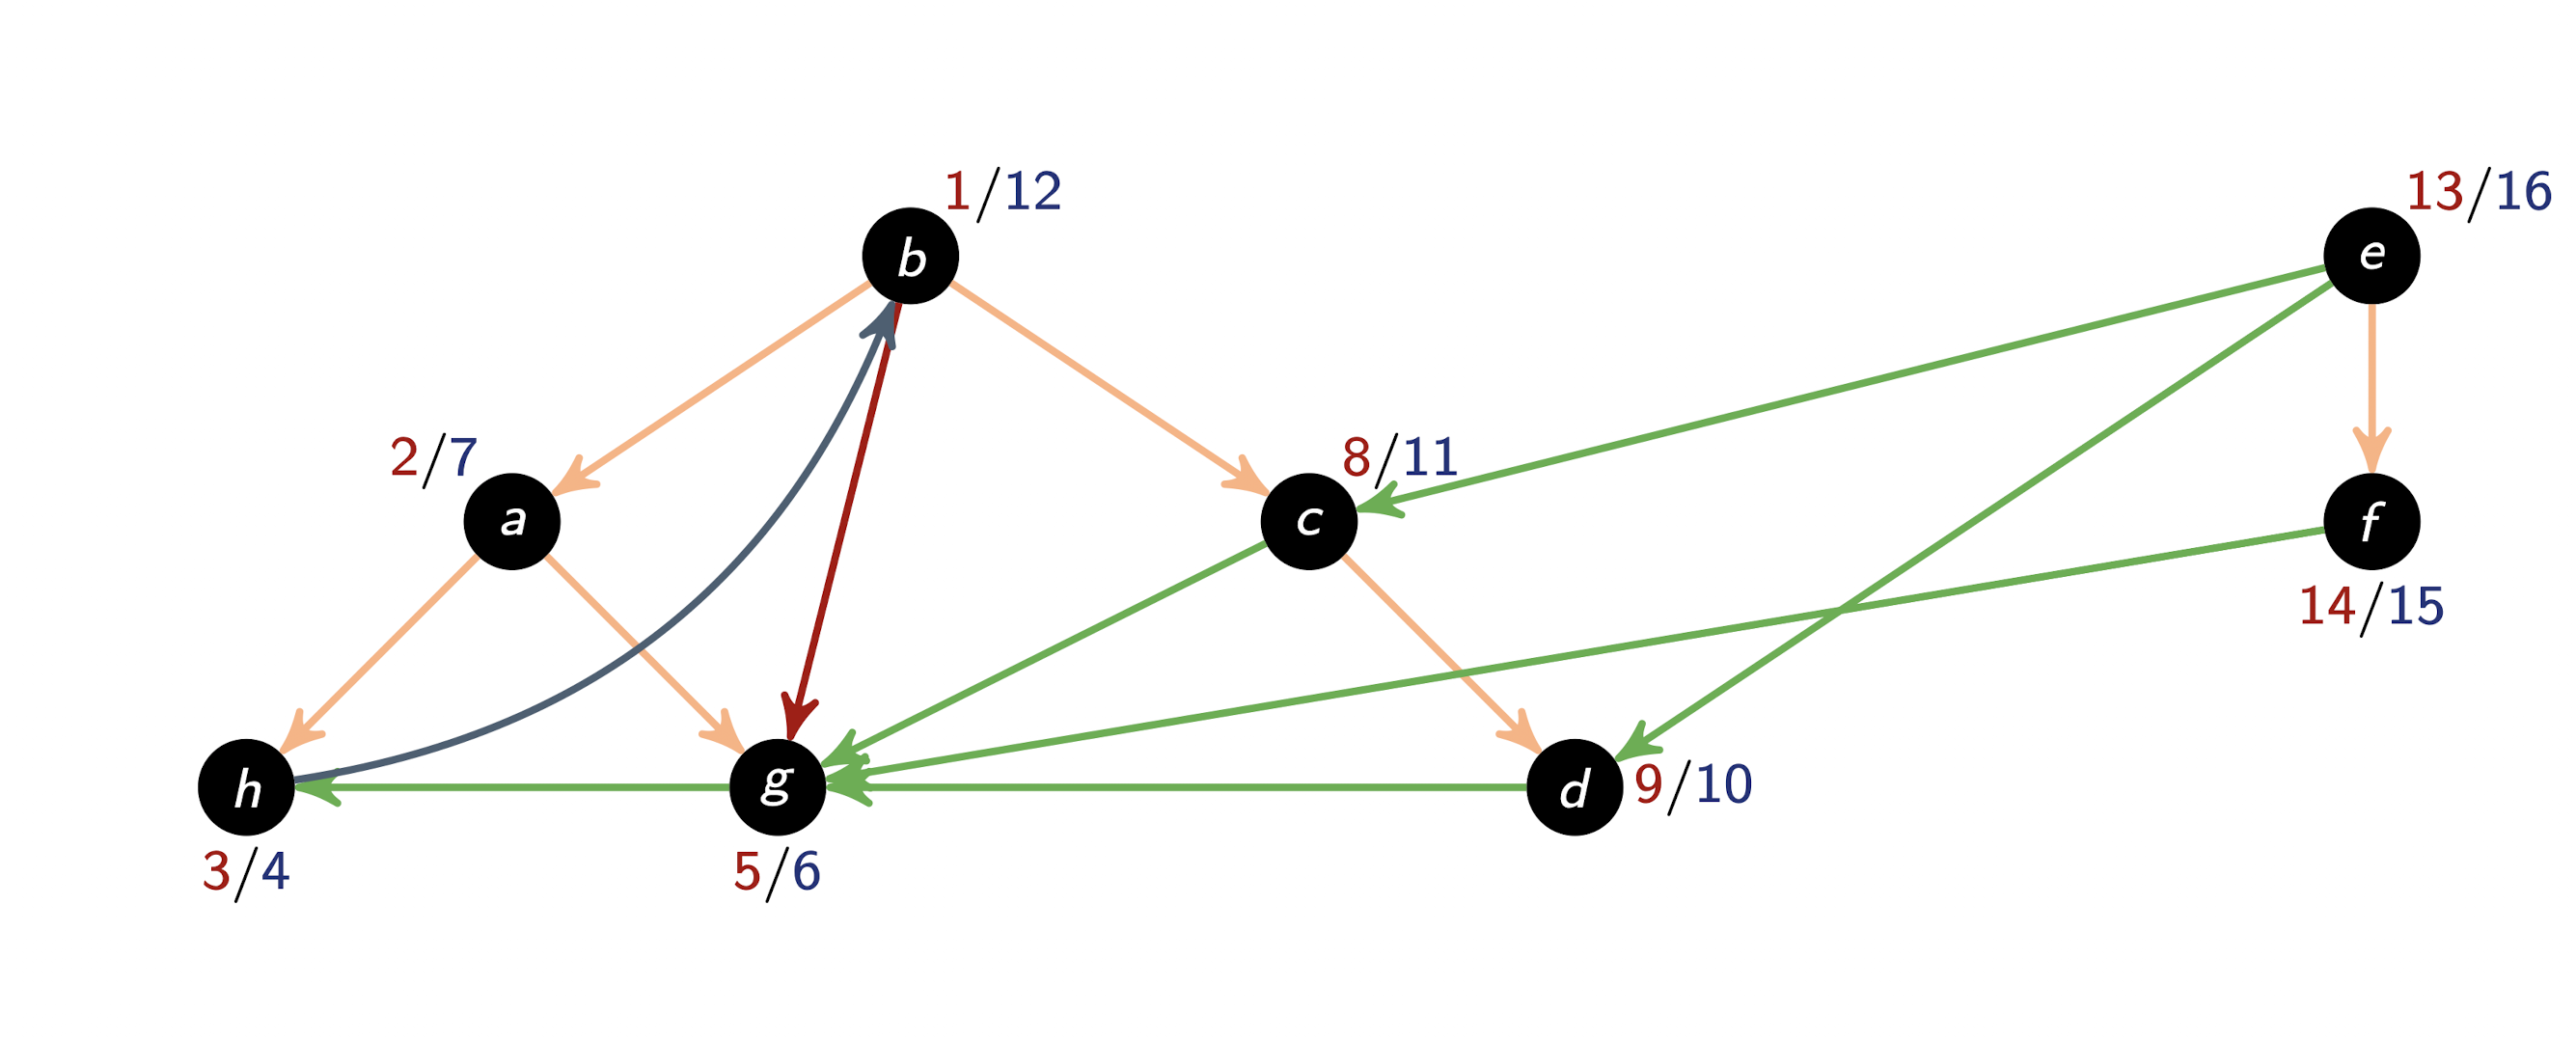
\includegraphics[width=\textwidth]{DFS}%
\endtcolorbox

\tcolorbox[mybox={Flow Network}]
We model the movement of flow through a network of edges, where each edge has a \textbf{capacity}—the maximum flow allowed. Our goal is to maximize the total flow from a \textbf{source} vertex $s$ to a \textbf{sink} vertex $t$.

\textbf{Flow Function:} A flow is a function $f : V \times V \to \mathbb{R}$ that satisfies:

\begin{enumerate}[noitemsep, topsep=0pt]
    \item \textbf{Capacity Constraint:} For all $u, v \in V$,
    \[
    0 \leq f(u, v) \leq c(u, v)
    \]
    where $c(u, v)$ is the capacity of edge $(u, v)$.
    
    \item \textbf{Flow Conservation:} For all $u \in V \setminus \{s, t\}$,
    \[
    \sum_{v \in V} f(v, u) = \sum_{v \in V} f(u, v)
    \]
    i.e., the total flow into $u$ equals the total flow out of $u$ (except for source and sink).
\end{enumerate}

\textbf{Value of the Flow:}
\[
|f| = \sum_{v \in V} f(s, v) - \sum_{v \in V} f(v, s)
\]
This represents the total net flow out of the source $s$.
\endtcolorbox

\tcolorbox[mybox={Ford-Fulkerson Method (1954)}]
The Ford-Fulkerson method finds the maximum flow from a source $s$ to a sink $t$ in a flow network $G = (V, E)$.

\textbf{Algorithm:}
\begin{enumerate}[noitemsep, topsep=0pt]
    \item Initialize flow $f(u, v) = 0$ for all $(u, v) \in E$.
    \item While there exists an \textbf{augmenting path} $p$ from $s$ to $t$ in the residual network $G_f$:
    \begin{itemize}
        \item Compute the \textbf{bottleneck capacity} $c_f(p)$ (the minimum residual capacity along $p$).
        \item Augment flow $f$ along $p$ by $c_f(p)$.
    \end{itemize}
\end{enumerate}

\textbf{Residual Network:} Given flow $f$, define residual capacity $c_f$ as:
\[
\resizebox{\textwidth}{!}{$
c_f(u, v) =
\begin{cases}
    c(u, v) - f(u, v) & \text{if } (u, v) \in E \\
    f(v, u) & \text{if } (v, u) \in E \\
    0 & \text{otherwise}
\end{cases}
$}
\]
Then the residual graph is $G_f = (V, E_f)$ where $E_f = \{(u, v) \in V \times V : c_f(u, v) > 0\}$.

\textbf{Cuts and Optimality:}
\begin{itemize}[noitemsep, topsep=0pt]
    \item A \textbf{cut} $(S, T)$ of the network is a partition of $V$ with $s \in S$, $t \in T$.
    
    \item The \textbf{flow across the cut} is:
    \[
    \resizebox{0.8\textwidth}{!}{$
    f(S, T) = \sum_{u \in S, v \in T} f(u, v) - \sum_{u \in T, v \in S} f(u, v)
    $}
    \]
    
    \item The \textbf{capacity of the cut} is:
    \[
    \resizebox{0.7\textwidth}{!}{$
    c(S, T) = \sum_{u \in S, v \in T} c(u, v)
    $}
    \]
    
    \item For any flow $f$ and any cut $(S, T)$, we have: $|f| \leq c(S, T)$.
\end{itemize}


\textbf{Max-Flow Min-Cut Theorem:} The value of the maximum flow equals the capacity of the minimum cut.\\
\textbf{Augmenting Path}
Is a path from the source to the sink in the residual graph such that every edge on the path has available capacity \\
\textbf{Time complexity:} \(\timecomplexity{\bigo(E|flow_{max}|)}\)
\endtcolorbox

\tcolorbox[mybox={Bipartite Graphs}]
A \textbf{bipartite graph} (or bigraph) is a graph $G = (U, V, E)$ whose vertices can be partitioned into two disjoint sets $U$ and $V$ such that every edge connects a vertex from $U$ to one in $V$.

\textbf{Properties:}
\begin{itemize}[noitemsep, topsep=0pt]
    \item $U$ and $V$ are called the \textit{parts} of the graph.
    \item Bipartiteness can be tested using BFS:
    \begin{itemize}[noitemsep, topsep=0pt]
        \item Label the source $s$ as \texttt{even}.
        \item During BFS, label each unvisited neighbor of a vertex with the opposite parity (\texttt{even} $\leftrightarrow$ \texttt{odd}).
        \item If a conflict arises (a vertex is visited twice with the same parity), the graph is not bipartite.
    \end{itemize}
\end{itemize}
 \textbf{Bipartite Match via Max-Flow}
\begin{itemize}
  \item \textbf{1. Add a source node} $s$ and connect it to all nodes in the left partition (say $U$) and do same for right part to sink.
  \item \textbf{2. For each edge} $(u, v)$ in the bipartite graph (with $u \in U$, $v \in V$), add a directed edge from $u$ to $v$.
  \item \textbf{3. Assign a capacity of 1} to all edges.
  \item \textbf{4. Run Ford–Fulkerson} from $s$ to $t$.
\end{itemize}
\endtcolorbox

\tcolorbox[mybox={Spanning Trees}]
\textbf{Spanning Tree:}  
A \emph{spanning tree} $T$ of an undirected graph $G = (V, E)$ is a subgraph that:
\begin{itemize}[noitemsep, topsep=0pt]
    \item Includes all vertices of $G$.
    \item Is a tree: connected and acyclic.
\end{itemize}

\textbf{Minimum Spanning Tree (MST):}  
An MST is a spanning tree of a weighted graph with the \emph{minimum total edge weight} among all spanning trees of the graph.

\textbf{Key Properties:}
\begin{itemize}[noitemsep, topsep=0pt]
    \item Every connected undirected graph has at least one MST.
    \item An MST connects all vertices using the lightest possible total edge weight without forming cycles.
\end{itemize}
\endtcolorbox
\tcolorbox[mybox={Prim’s Algorithm}]
\textbf{Goal:} Find a Minimum Spanning Tree (MST) of a connected, weighted undirected graph.

\textbf{Idea:}
\begin{enumerate}[noitemsep, topsep=0pt]
    \item Start from an arbitrary root vertex $r$.
    \item Maintain a growing tree $T$, initialized with $r$.
    \item Repeatedly add the minimum-weight edge that connects a vertex in $T$ to a vertex outside $T$.
\end{enumerate}

\textbf{Data Structures:}
Uses a min-priority queue to select the next lightest edge crossing the cut.

\noindent % Prevents indentation if at the start of a paragraph
\resizebox{\linewidth}{!}{%
\begin{minipage}{1.25\linewidth}
\begin{algorithmic}[1]
    \Procedure{Prim}{$G, w, r$}
        \State let $Q$ be a new min-priority queue
        \For{\textbf{each} $u \in G.V$}
            \State $u.\text{key} \gets \infty$
            \State $u.\pi \gets \text{NIL}$
            \State \Call{Insert}{$Q, u$}
        \EndFor
        \State \Call{Decrease-Key}{$Q, r, 0$}
        \While{$Q \neq \emptyset$}
            \State $u \gets \Call{Extract-Min}{Q}$
            \For{\textbf{each} $v \in G.\text{adj}[u]$}
                \If{$v \in Q$ and $w(u, v) < v.\text{key}$}
                    \State $v.\pi \gets u$
                    \State \Call{Decrease-Key}{$Q, v, w(u, v)$}
                \EndIf
            \EndFor
        \EndWhile
    \EndProcedure
\end{algorithmic}
\end{minipage}%
}

\textbf{Runtime:} \timecomplexity{$\Theta((ElogV)$} \\ $\Theta(E+VlogV)$ with Fibonacci heaps.
\endtcolorbox

\tcolorbox[mybox={Kruskal’s Algorithm}]
\textbf{Goal:} Find a Minimum Spanning Tree (MST) in a connected, weighted undirected graph.

\textbf{Idea:}
\begin{enumerate}[noitemsep, topsep=0pt]
    \item Start with an empty forest $A$ (each vertex is its own tree).
    \item Sort all edges in non-decreasing order of weight.
    \item For each edge $(u, v)$, if $u$ and $v$ are in different trees (i.e., no cycle is formed), add the edge to $A$.
    \item Use a disjoint-set (Union-Find) data structure to efficiently check and merge trees.
\end{enumerate}

\noindent % Prevents indentation if at the start of a paragraph
\resizebox{\linewidth}{!}{%
\begin{minipage}{1.25\linewidth}
\begin{algorithmic}[1]
    \Procedure{Kruskal}{$G, w$}
        \State $A \gets \emptyset$
        \For{\textbf{each} $v \in G.V$}
            \State \Call{Make-Set}{$v$}
        \EndFor
        \State sort the edges of $G.E$ into non-decreasing order by weight $w$
        \For{\textbf{each} $(u, v) \in$ sorted edge list}
            \If{\Call{Find-Set}{$u$} $\neq$ \Call{Find-Set}{$v$}}
                \State $A \gets A \cup \{(u, v)\}$
                \State \Call{Union}{$u, v$}
            \EndIf
        \EndFor
        \State \Return $A$
    \EndProcedure
\end{algorithmic}
\end{minipage}%
}

\textbf{Runtime:} \timecomplexity{$\Theta(|E| \log |E|)$} due to sorting, plus nearly linear time for Union-Find operations (with union by rank and path compression).
\endtcolorbox
\tcolorbox[mybox={Edge Disjoint Paths using Max Flow}]
You can use the Max-Flow algorithm to find all edge-disjoint paths from a source to a sink by assigning a capacity of $1$ to every edge and running Ford–Fulkerson.  
The maximum flow value will be equal to the number of edge-disjoint $s$–$t$ paths.
\endtcolorbox


\tcolorbox[mybox={Bellman-Ford Algorithm}]
\textbf{Goal:} Compute shortest paths from a single source $s$ to all other vertices in a weighted graph $G = (V, E)$, allowing negative edge weights.

\textbf{Key Idea:}
\begin{itemize}[noitemsep, topsep=0pt]
    \item Relax all edges repeatedly (up to $|V| - 1$ times).
    \item After that, check for negative-weight cycles: if we can still relax an edge, a negative cycle exists.
\end{itemize}


\textbf{Initialization:}
\noindent % Prevents indentation if at the start of a paragraph
\resizebox{\linewidth}{!}{%
\begin{minipage}{1.25\linewidth}
\begin{algorithmic}[1]
    \Procedure{Init-Single-Source}{$G, s$}
        \For{\textbf{each} $v \in G.V$}
            \State $v.d \gets \infty$ \Comment{distance estimate}
            \State $v.\pi \gets \text{NIL}$ \Comment{predecessor}
        \EndFor
        \State $s.d \gets 0$
    \EndProcedure
\end{algorithmic}
\end{minipage}%
}

\textbf{Relaxation:}
\noindent % Prevents indentation if at the start of a paragraph
\resizebox{\linewidth}{!}{%
\begin{minipage}{1.25\linewidth}
\begin{algorithmic}[1]
    \Procedure{Relax}{$u, v, w$}
        \If{$v.d > u.d + w(u, v)$}
            \State $v.d \gets u.d + w(u, v)$
            \State $v.\pi \gets u$
        \EndIf
    \EndProcedure
\end{algorithmic}
\end{minipage}%
}

\textbf{Main Algorithm:\\}
\noindent % Prevents indentation if at the start of a paragraph
\resizebox{\linewidth}{!}{%
\begin{minipage}{1.25\linewidth}
\begin{algorithmic}[1]
    \Procedure{Bellman-Ford}{$G, w, s$}
        \State \Call{Init-Single-Source}{$G, s$}
        \For{$i \gets 1$ \textbf{to} $|G.V| - 1$}
            \For{\textbf{each} edge $(u, v) \in G.E$}
                \State \Call{Relax}{$u, v, w$}
            \EndFor
        \EndFor
        \For{\textbf{each} edge $(u, v) \in G.E$}
            \If{$v.d > u.d + w(u, v)$}
                \State \Return \textbf{false} \Comment{Negative-weight cycle detected}
            \EndIf
        \EndFor
        \State \Return \textbf{true}
    \EndProcedure
\end{algorithmic}
\end{minipage}%
}


\textbf{Runtime:} \timecomplexity{$\Theta(|V||E|)$} \\
\textbf{Handles:} Negative weights (but no negative cycles)
\endtcolorbox

\tcolorbox[mybox={Dijkstra’s Algorithm}]
\textbf{Goal:} Compute the shortest paths from a single source $s$ to all other vertices in a weighted graph $G = (V, E)$ with non-negative edge weights.

\textbf{Key Idea:}
\begin{itemize}[noitemsep, topsep=0pt]
    \item Greedily grow a set $S$ of vertices with known shortest paths.
    \item At each step, pick the vertex $u \notin S$ with the smallest tentative distance $u.d$.
    \item Relax all edges $(u, v)$ from $u$ to update distance estimates.
\end{itemize}
\textbf{Pseudocode:}
\resizebox{\linewidth}{!}{%
\begin{minipage}{1.25\linewidth}
\begin{algorithmic}[1]
   \Procedure{Dijkstra}{$G, w, s$}
    \State \Call{Init-Single-Source}{$G, s$}
    \State $S \gets \emptyset$
    \State $Q \gets G.V$ \Comment{insert all vertices into priority queue $Q$}
      \While{$Q \neq \emptyset$}
           \State $u \gets$ \Call{Extract-Min}{$Q$}
          \State $S \gets S \cup \{u\}$
         \For{each $v \in \text{Adj}[u]$}
                \State \Call{Relax}{$u, v, w$}
         \EndFor
        \EndWhile
    \EndProcedure
\end{algorithmic}
\end{minipage}%
}
\textbf{Runtime:} \timecomplexity{$\Theta(|E| \log |V|)$}
\endtcolorbox
\tcolorbox[mybox={HTable}]
Hash tables are a data structure that use a function $h(k)$ mapping keys to indices in the range $1$ to $p$, such that each element is stored at index $h(k)$.  
Collisions are managed using chaining (linked lists), leading to:
\begin{itemize}
  \item \textbf{Insertion} \timecomplexity{$\bigo(1)$}
  \item \textbf{Search} \timecomplexity{$\bigo(1)$} E[x]: \timecomplexity{$\bigo(n/m)$}
  \item \textbf{Deletion} \timecomplexity{$\bigo(1)$ }
  \item \textbf{Collisions expected} for m entries and n insertions (uniformly random hash function): \(\frac{n^2}{m}\)
\end{itemize}
\endtcolorbox

\tcolorbox[mybox={Randomized caching}]
\begin{itemize}
    \item Each page is marked (if used recently) or unmarked.
    \item On miss, evict random unmarked page.
    \item \textbf{Competitive ratio:} \(2H(k) \approx \bigo(logk)\) (nearly optimal, no randomized algorithm can beat $H(k)$).
\end{itemize}
\endtcolorbox

\tcolorbox[mybox={Deterministic caching}]
\textbf{LRU/FIFO}:\\
Competitive ratio = $k(\text{cache size})$.\\
\textbf{LFU/LIFO}:\\
Unbounded competitive ratio (arbitrary bad).
\endtcolorbox

\tcolorbox[mybox={The Hiring Problem}]
\textbf{Problem:} We interview $n$ candidates for a position, one by one in random order. After each interview, we decide immediately whether to hire the candidate. We want to compute the expected number of times we hire someone (i.e., when they are better than all previous candidates).


\textbf{Indicator Random Variable:}  
Given a sample space and an event $A$, the indicator random variable for $A$ is defined as:
\[
I\{A\} =
\begin{cases}
    1 & \text{if } A \text{ occurs}, \\
    0 & \text{if } A \text{ does not occur}.
\end{cases}
\]
Then:  
\[
\mathbb{E}[I\{A\}] = P(A)
\]


\textbf{Expected Number of Hires:}  
Let $X$ be the total number of hires. Define $X = \sum_{i=1}^n I_i$, where $I_i = 1$ if the $i$-th candidate is hired (i.e., better than all previous $i - 1$), and 0 otherwise.

\begin{equation}
    \begin{split}
    \mathbb{E}[X] = \sum_{i=1}^n \mathbb{E}[I_i] & = \sum_{i=1}^n \frac{1}{i} = H_n \\[-1mm]
    & = logn + \Theta(1)
    \end{split}
\end{equation}

\textbf{Conclusion:}  
The expected number of hires is \timecomplexity{$\Theta(\log n)$}, even though there are $n$ candidates.
\endtcolorbox

\tcolorbox[mybox={Secretary problem}]
$n$ candidates arrive in random order, we can hire at most 1 and want best one.
\begin{itemize}
    \item Hire 1st candidate: \\Pr[success] = $1/n$.
    \item Observe first n/2 and select first better: Pr[success] $\geq 1/4$
    \item Optimal: observe n/e candidates and select first better:\\ Pr[success] $\geq 1/e \approx 36.8\%$
\end{itemize}
\endtcolorbox

\tcolorbox[mybox={Quick Sort}]
\textbf{Quick Sort} is a divide-and-conquer algorithm with the following steps:

\begin{enumerate}[noitemsep, topsep=0pt]
    \item \textbf{Divide:} Partition $A[p, \dots, r]$ into two (possibly empty) subarrays $A[p, \dots, q-1]$ and $A[q+1, \dots, r]$ such that each element in the first subarray is $\leq A[q]$ and each element in the second subarray is $\geq A[q]$.
    \item \textbf{Conquer:} Recursively sort the two subarrays by calling Quick Sort on them.
    \item \textbf{Combine:} No work is needed to combine the subarrays since the sorting is done in-place.
\end{enumerate}

\noindent % Prevents indentation if at the start of a paragraph
\resizebox{\linewidth}{!}{%
\begin{minipage}{1.25\linewidth}
\begin{algorithmic}[1]
    \Procedure{Partition}{$A, p, r$} \timecomplexity{$\bigo(n)$}
        \State $x \gets A[r]$
        \State $i \gets p - 1$
        \For{$j \gets p$ \textbf{to} $r - 1$}
            \If{$A[j] \leq x$}
                \State $i \gets i + 1$
                \State exchange $A[i]$ with $A[j]$
            \EndIf
        \EndFor
        \State exchange $A[i + 1]$ with $A[r]$
        \State \Return $i + 1$
    \EndProcedure
\end{algorithmic}
\end{minipage}%
}

\vspace{1em} % Add some vertical space between algorithms for better separation

\noindent % Prevents indentation if at the start of a paragraph
\resizebox{\linewidth}{!}{%
\begin{minipage}{1.25\linewidth}
\begin{algorithmic}[1]
    \Procedure{Quick-Sort}{$A, p, r$} \timecomplexity{$\bigo(nlogn)$}
        \If{$p < r$}
            \State $q \gets \Call{Partition}{A, p, r}$
            \State \Call{Quick-Sort}{$A, p, q - 1$}
            \State \Call{Quick-Sort}{$A, q + 1, r$}
        \EndIf
    \EndProcedure
\end{algorithmic}
\end{minipage}%
}

\vspace{1em} % Add some vertical space between algorithms for better separation

\noindent % Prevents indentation if at the start of a paragraph
\resizebox{\linewidth}{!}{%
\begin{minipage}{1.25\linewidth}
\begin{algorithmic}[1]
    \Procedure{Randomized-Partition}{$A, p, r$}
        \State $i \gets \Call{Random}{p, r}$
        \State exchange $A[r]$ with $A[i]$
        \State \Return \Call{Partition}{$A, p, r$}
    \EndProcedure \timecomplexity{$\Theta(nlogn)$}
\end{algorithmic}
\end{minipage}%
}

\vspace{1em} % Add some vertical space between algorithms for better separation

\noindent % Prevents indentation if at the start of a paragraph
\resizebox{\linewidth}{!}{%
\begin{minipage}{1.25\linewidth}
\begin{algorithmic}[1]
    \Procedure{Randomized-Quick-Sort}{$A, p, r$}
        \If{$p < r$}
            \State $q \gets \Call{Randomized-Partition}{A, p, r}$
            \State \Call{Quick-Sort}{$A, p, q - 1$}
            \State \Call{Quick-Sort}{$A, q + 1, r$}
        \EndIf
    \EndProcedure
\end{algorithmic}
\end{minipage}%
}
\textbf{Random Runtime:} \timecomplexity{$\Theta(nlogn)$} \\
\textbf{Worst Runtime:} \timecomplexity{$\Theta(n^2)$}

\tcblower

\textbf{Probability} to compare elements of A $z_i$ with $z_j$:
\begin{itemize}
    \item If x the pivot $z_i < x < z_j$ then $Pr = 0$.
    \item Else $Pr = \frac{2}{j-i+1}$
\end{itemize}

\endtcolorbox

\tcolorbox[mybox={Online Algorithms}]
An \textbf{online algorithm} processes its input piece-by-piece in a serial fashion, i.e., it does not have access to the entire input from the start. Instead, it must make decisions based only on the current and past inputs without knowledge of future inputs.


\textbf{Characteristics:}
\begin{itemize}[noitemsep, topsep=0pt]
    \item Decisions are made in real-time.
    \item Cannot revise past decisions once new input arrives.
    \item Often evaluated using \textit{competitive analysis}, comparing performance to an optimal offline algorithm.
\end{itemize}
\textbf{Competitive Ratio:}  
If $C_{\text{online}}$ is the cost incurred by the online algorithm and $C_{\text{opt}}$ is the cost incurred by an optimal offline algorithm, then the competitive ratio is defined as:
\[
\text{Competitive Ratio} = \max_{\text{input}} \frac{C_{\text{online}}}{C_{\text{opt}}}
\]

An algorithm is said to be $r$-competitive if this ratio is at most $r$ for all inputs.
\endtcolorbox
\tcolorbox[mybox={Weighted Majority Algorithm}]
The \textbf{Weighted Majority Algorithm (WMA)} is an online learning algorithm that maintains a set of "experts" (prediction strategies), each assigned a weight. The algorithm predicts based on a weighted vote of the experts and penalizes those who make incorrect predictions.


\textbf{Setup:}
\begin{itemize}[noitemsep, topsep=0pt]
    \item $n$ experts, each with an initial weight $w_i \gets 1$.
    \item At each time step $t$, each expert $i$ makes a prediction.
    \item The algorithm makes its own prediction based on a weighted majority.
    \item After the outcome is revealed, experts that predicted incorrectly are penalized by multiplying their weight by a factor $\beta \in (0, 1)$.
\end{itemize}


\textbf{Guarantees:}  
If there is an expert that makes at most $m$ mistakes, then the number of mistakes made by the algorithm is at most:
\[
M \leq (1 + \log n) \cdot m
\]
(up to constant factors depending on $\beta$)


\textbf{Use cases:} Binary prediction problems, stock forecasting, game playing.
\endtcolorbox
\tcolorbox[mybox={Hedge Algorithm}]
The \textbf{Hedge Algorithm} generalizes Weighted Majority to handle real-valued losses and probabilistic predictions. It is used in adversarial multi-armed bandit and online optimization settings.


\textbf{Setup:}
\begin{itemize}[noitemsep, topsep=0pt]
    \item $n$ actions (or experts), each with weight $w_i^{(t)}$ at round $t$.
    \item At each time step, the algorithm picks a probability distribution $p^{(t)}$ over actions, where:
    \[
    p_i^{(t)} = \frac{w_i^{(t)}}{\sum_j w_j^{(t)}}
    \]
    \item After observing losses $\ell_i^{(t)} \in [0,1]$, weights are updated as:
    \[
    w_i^{(t+1)} = w_i^{(t)} \cdot e^{-\eta \ell_i^{(t)}}
    \]
    where $\eta > 0$ is the learning rate.
\end{itemize}


\textbf{Guarantees:}  
For any expert $i$, the regret after $T$ rounds is bounded by:
\[
\text{Regret} \leq \eta T + \frac{\log n}{\eta}
\]
Setting $\eta = \sqrt{\frac{\log n}{T}}$ gives regret of order $O(\sqrt{T \log n})$.


\textbf{Use cases:} Adversarial learning, portfolio selection, online convex optimization.
\endtcolorbox


\end{multicols}


\end{document}
